\chapter{Điều kiện và vòng lặp trong workflow}

\section{Giới thiệu}

Các workflow thực tế thường yêu cầu logic phức tạp hơn việc thực hiện các bước một cách tuần tự. Đôi khi bạn cần thực hiện các tác vụ khác nhau dựa trên điều kiện, hoặc lặp lại một tác vụ nhiều lần. Chương này sẽ giới thiệu cách sử dụng các nút điều kiện và vòng lặp trong n8n để tạo các workflow linh hoạt và mạnh mẽ.

\section{If, Switch, Merge Node}

\subsection{IF Node - Điều kiện cơ bản}

IF Node là nút điều kiện cơ bản trong n8n, cho phép workflow rẽ nhánh dựa trên các điều kiện được định nghĩa.

\subsubsection{Cách hoạt động của IF Node}

IF Node đánh giá một hoặc nhiều điều kiện và định tuyến dữ liệu đến ``True'' hoặc ``False'' dựa trên kết quả đánh giá:

\begin{figure}[htbp]
    \centering
    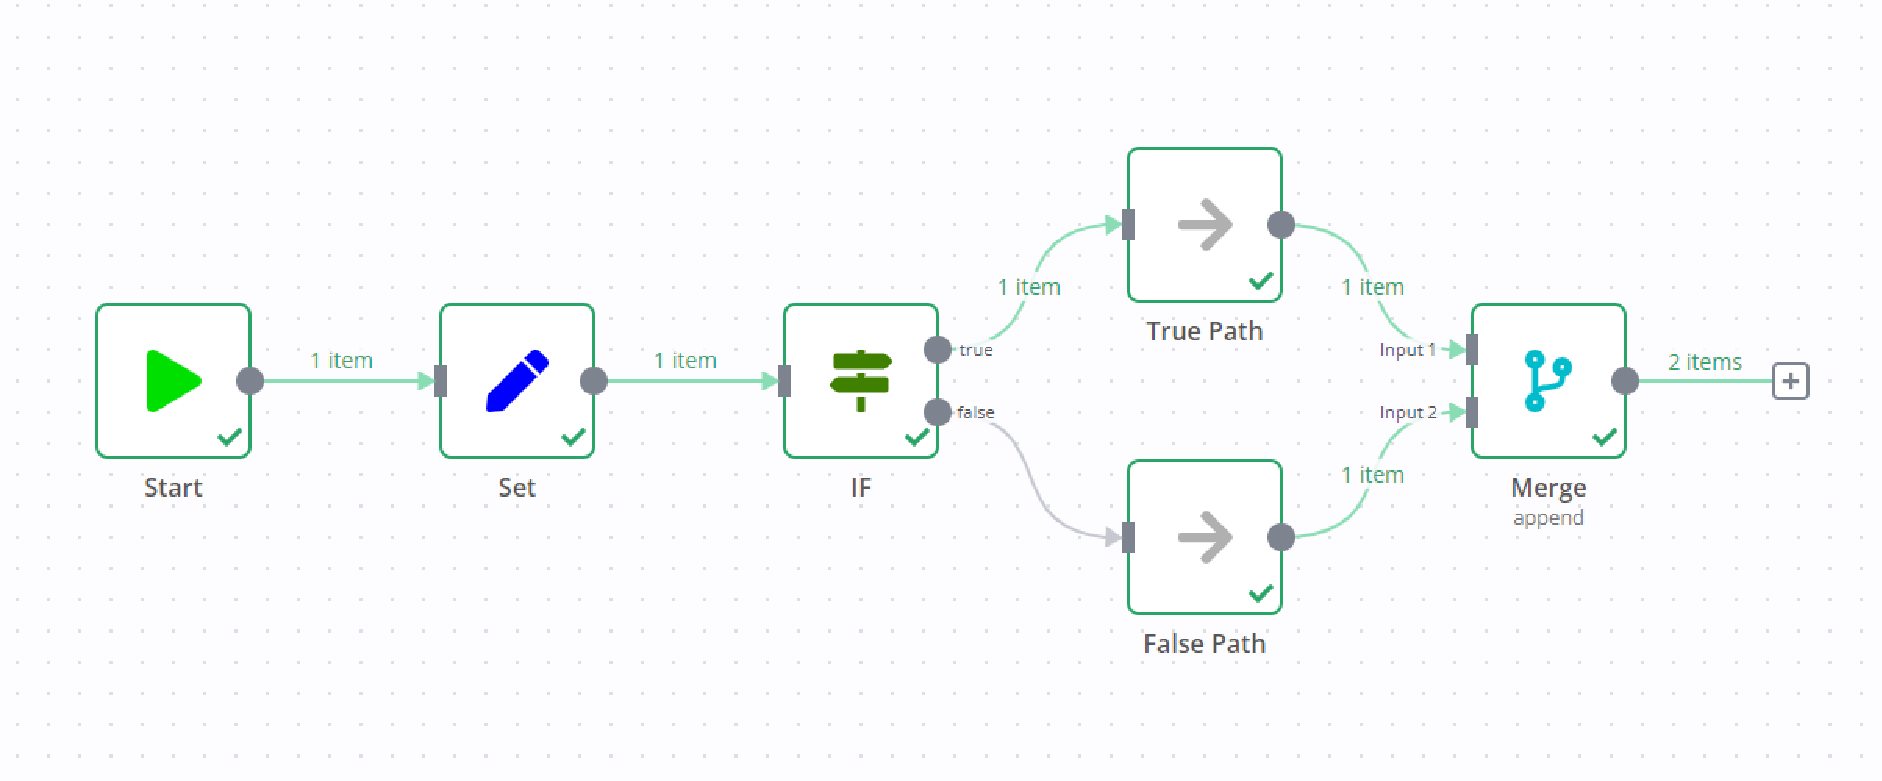
\includegraphics[width=1\linewidth]{Chap1-7/if-merge-node.pdf}
\end{figure} 

\newpage

\subsubsection{Cấu hình IF Node}

\begin{enumerate}
  \item \textbf{Thêm IF Node vào workflow}:
  \begin{itemize}
    \item Tìm và thêm ``IF'' từ thư viện nút.
  \end{itemize}

  \item \textbf{Thiết lập điều kiện}:
  \begin{itemize}
    \item Mỗi điều kiện bao gồm ba thành phần: Giá trị 1, Toán tử so sánh, Giá trị 2.
    \item Ví dụ: \texttt{\{\{\$json["status"]\}\}} \texttt{equals} \texttt{"success"}.
  \end{itemize}
$\Rightarrow$  \textit{Đoạn này với từng điều kiện là text hay số thì phải chọn toán tử so sánh tương ứng.}
  \item \textbf{Kết hợp nhiều điều kiện}:
  \begin{itemize}
    \item Bạn có thể thêm nhiều điều kiện và kết hợp chúng bằng ``AND'' hoặc ``OR''.
    \item AND: Tất cả các điều kiện phải đúng.
    \item OR: Chỉ cần một điều kiện đúng.
  \end{itemize}
\end{enumerate}

\subsubsection{Ví dụ: Xử lý phản hồi API}

Giả sử bạn đang gọi một API để lấy dữ liệu thời tiết và muốn thông báo khi nhiệt độ vượt quá ngưỡng. Truy cập \href{https://www.weatherapi.com/my/}{openweathermap} để lấy api thời tiết miễn phí. 

\begin{figure}[htbp]
    \centering
    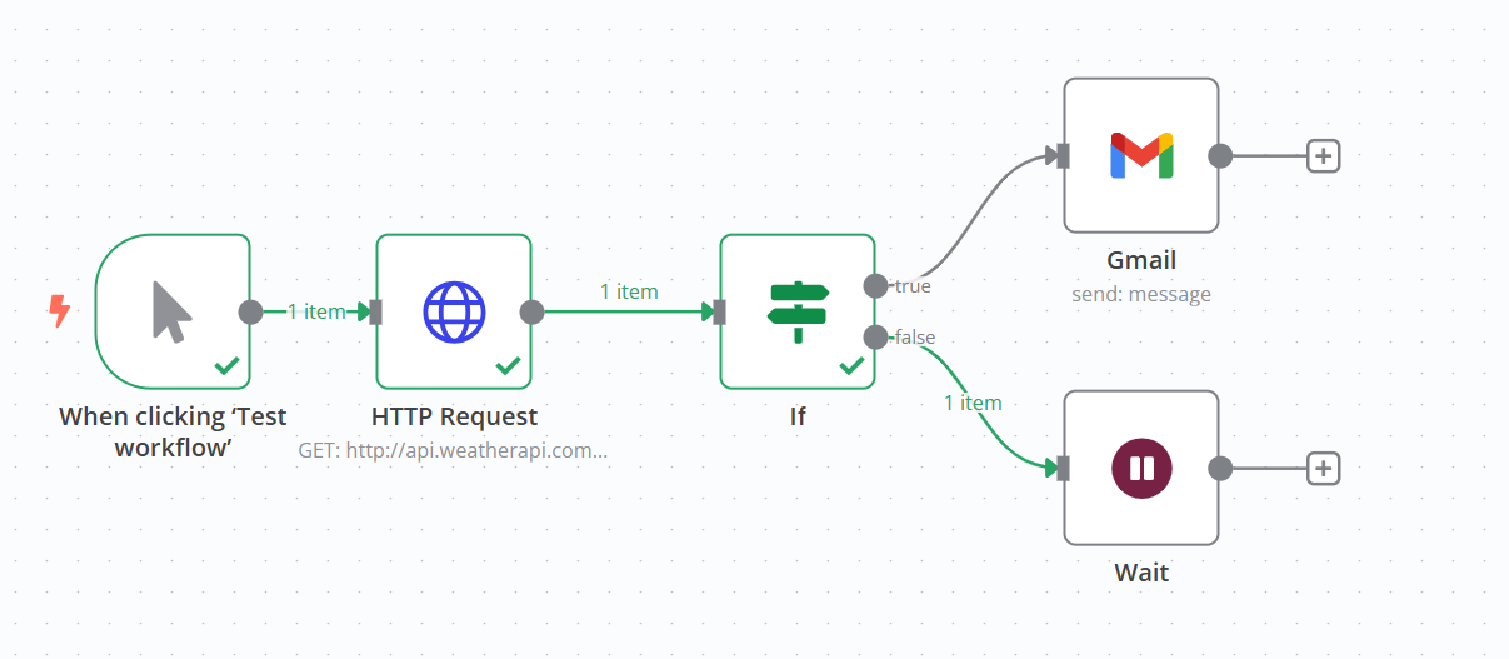
\includegraphics[width=1\linewidth]{Chap1-7/weather.pdf}
    \caption{Workflow thông báo thời tiết}
\end{figure} 

Cấu hình IF Node:

\begin{itemize}
  \item Điều kiện: \texttt{\{\{\$json["temperature"]\}\}} \texttt{larger} \texttt{30}
  \item Nếu thời tiết nóng hơn 30°C, gửi email cảnh báo.
\end{itemize}

\newpage

\subsection{Switch Node - Nhiều nhánh điều kiện}

Switch Node mở rộng khái niệm của IF Node bằng cách cho phép nhiều đường dẫn khác nhau, không chỉ True/False.
\subsubsection{Cách hoạt động của Switch Node}

Switch Node đánh giá một giá trị và định tuyến dữ liệu theo nhiều nhánh khác nhau dựa trên kết quả.

\begin{figure}[htbp]
    \centering
    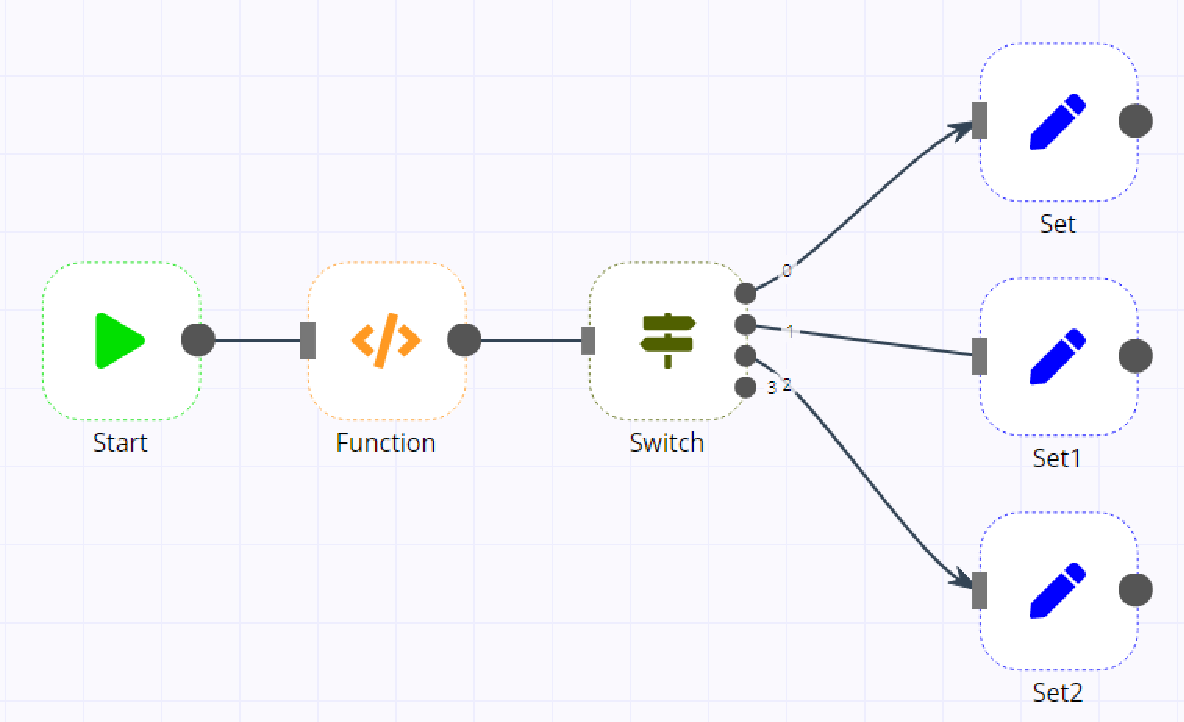
\includegraphics[width=1\linewidth]{Chap1-7/switch_node.pdf}
\end{figure}

\subsubsection{Cấu hình Switch Node}

\begin{enumerate}
  \item \textbf{Thêm Switch Node vào workflow}:
  \begin{itemize}
    \item Tìm và thêm ``Switch'' từ thư viện nút.
  \end{itemize}

  \item \textbf{Thiết lập giá trị đánh giá}:
  \begin{itemize}
    \item Chọn trường dữ liệu để đánh giá (Value to Switch On).
    \item Ví dụ: \texttt{\{\{\$json["status"]\}\}}
  \end{itemize}

  \item \textbf{Định nghĩa các nhánh đầu ra}:
  \begin{itemize}
    \item Thêm trường Output cho mỗi giá trị có thể.
    \item Đặt tên cho mỗi nhánh.
    \item Xác định giá trị khớp.
  \end{itemize}
\end{enumerate}

\newpage
\subsubsection{Ví dụ: Phân loại khách hàng}

\begin{figure}[htbp]
    \centering
    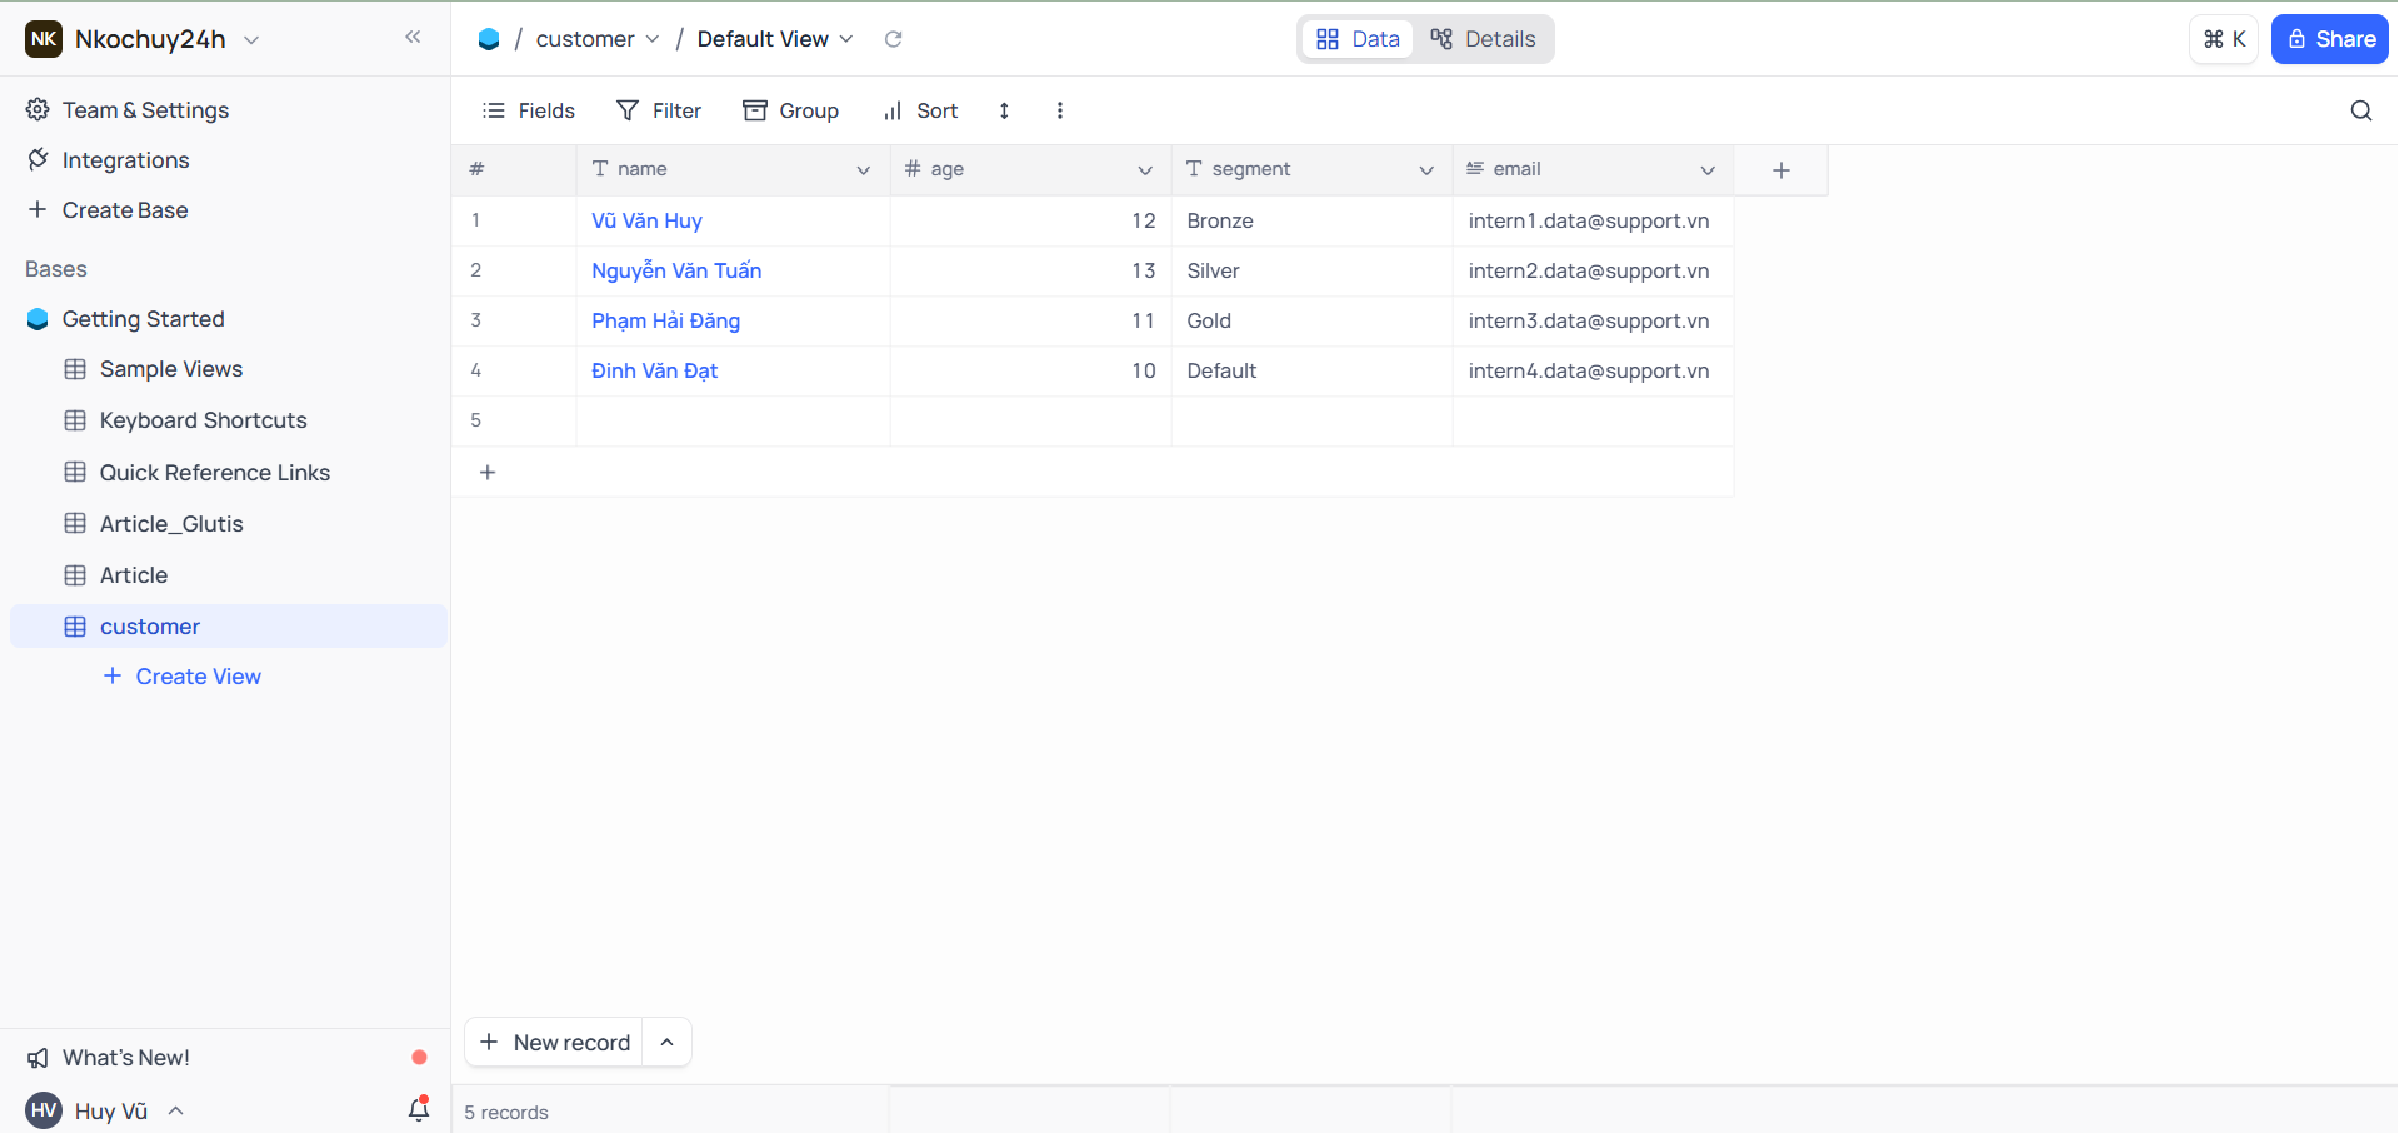
\includegraphics[width=1\linewidth]{Chap1-7/segment_db.pdf}
    \caption{Database chia phân loại khách hàng}
\end{figure}

Xây dựng workflow phân loại khách hàng dựa trên cấp độ thành viên:

\begin{figure}[htbp]
    \centering
    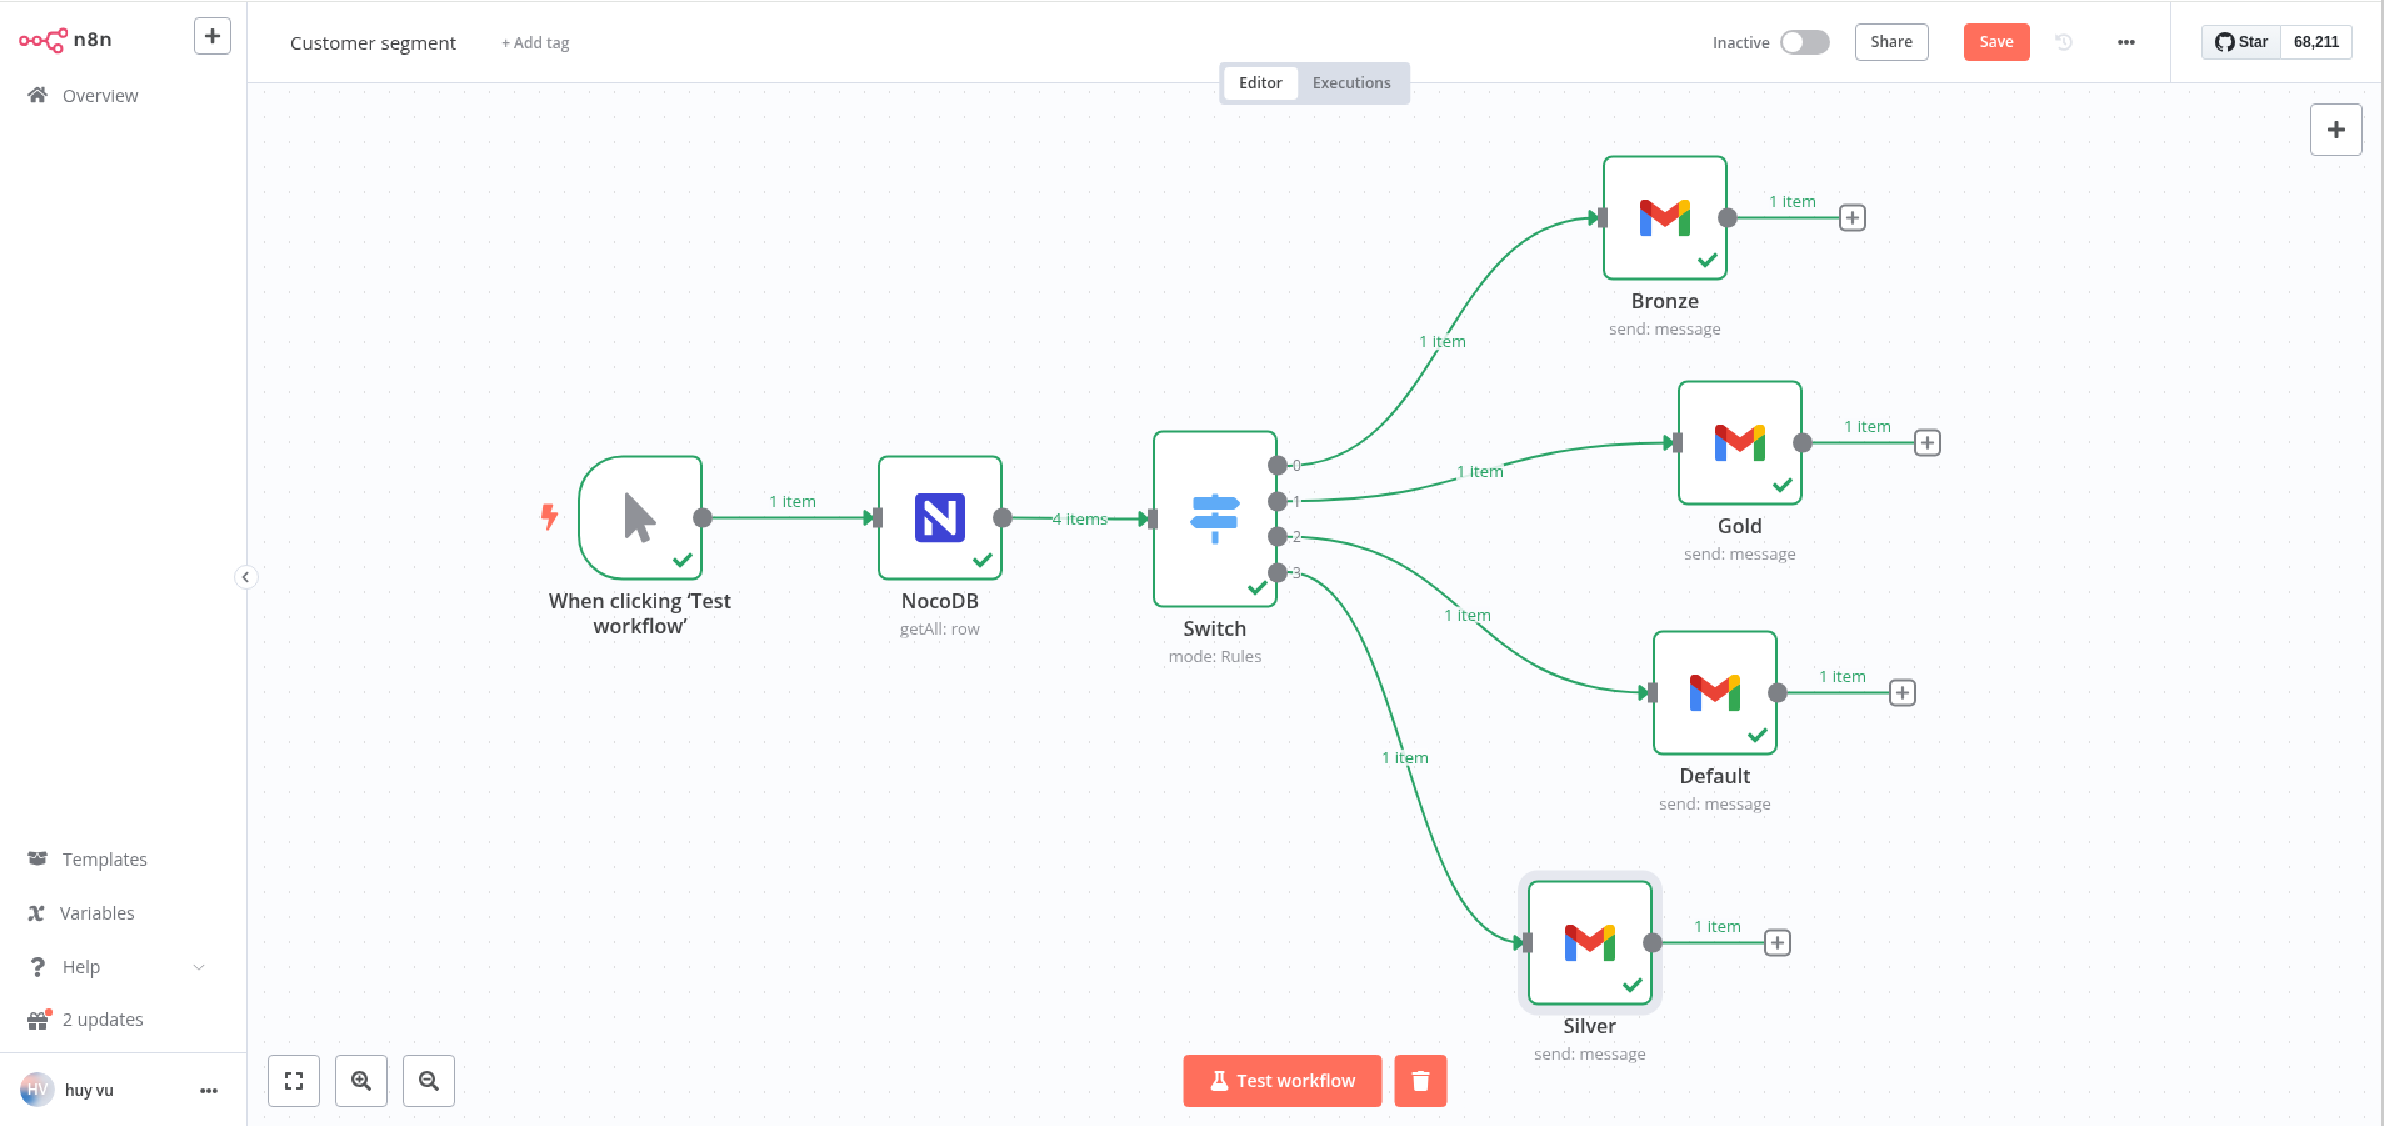
\includegraphics[width=1\linewidth]{Chap1-7/segment.pdf}
    \caption{Gửi email chăm sóc theo phân khúc khách hàng}
\end{figure}

Cấu hình Switch Node:
\begin{itemize}
  \item Value to Switch On: \texttt{\{\{\$json["membership\_level"]\}\}}
  \item Output 1: Name ``Bronze'', Value ``bronze''
  \item Output 2: Name ``Silver'', Value ``silver''
  \item Output 3: Name ``Gold'', Value ``gold''
  \item Default Output: For unmatched values
\end{itemize}

\subsection{Merge Node - Kết hợp dữ liệu từ nhiều nhánh}

Sau khi chia workflow thành nhiều nhánh với IF hoặc Switch, bạn thường cần kết hợp chúng lại để tiếp tục xử lý. Đây là lúc Merge Node phát huy tác dụng.

\subsubsection{Cách hoạt động của Merge Node}

Merge Node kết hợp dữ liệu từ nhiều nhánh thành một luồng duy nhất theo nhiều cách khác nhau.

\begin{figure}[htbp]
    \centering
    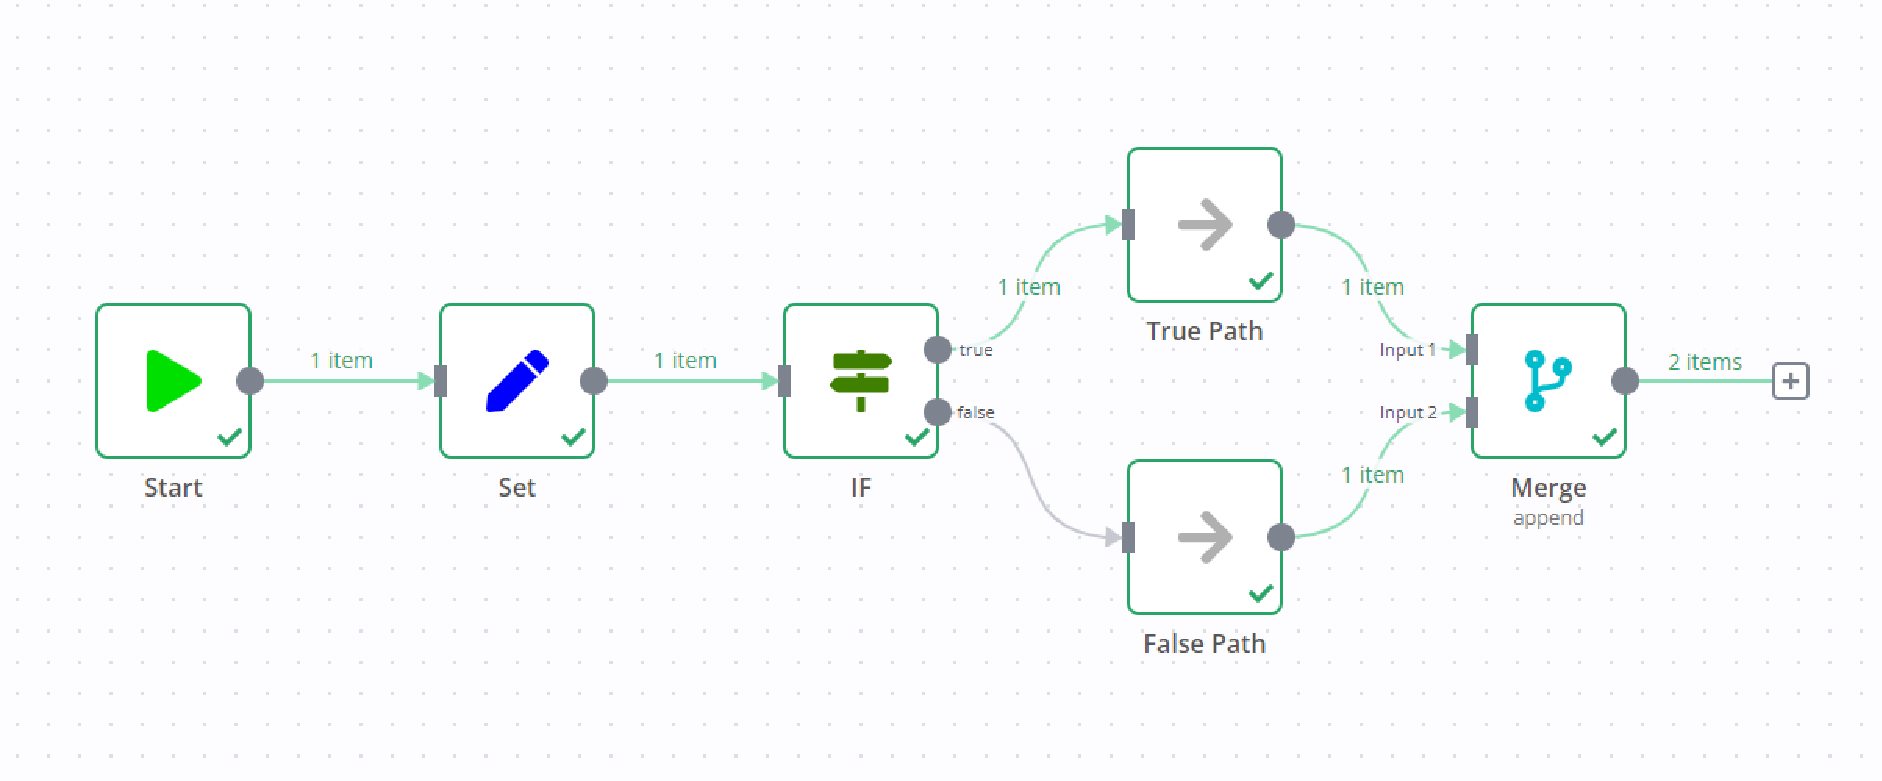
\includegraphics[width=1\linewidth]{Chap1-7/merge_node.pdf}
\end{figure} 

\subsubsection{Chế độ hoạt động của Merge Node}

\begin{enumerate}
  \item \textbf{Chế độ Append (Nối)}:
  \begin{itemize}
    \item Ghép các mục từ tất cả các đầu vào thành một mảng.
    \item Hữu ích khi bạn muốn xử lý tất cả các mục cùng một lúc.
  \end{itemize}

  \item \textbf{Chế độ Passthrough (Chuyển tiếp)}:
  \begin{itemize}
    \item Chuyển tiếp dữ liệu từ nút đầu tiên được kích hoạt.
    \item Hữu ích cho các tình huống ``race condition'' khi bạn chỉ muốn xử lý kết quả nhanh nhất.
  \end{itemize}

  \item \textbf{Chế độ Wait (Chờ đợi)}:
  \begin{itemize}
    \item Chờ tất cả các đầu vào trước khi xử lý.
    \item Có thể định cấu hình thêm để chỉ xử lý những đầu vào cụ thể.
  \end{itemize}
\end{enumerate}

\subsubsection{Ví dụ: Thu thập dữ liệu từ nhiều nguồn}

Thu thập dữ liệu sản phẩm từ nhiều API, sau đó tổng hợp thành một báo cáo:

\begin{figure}[htbp]
    \centering
    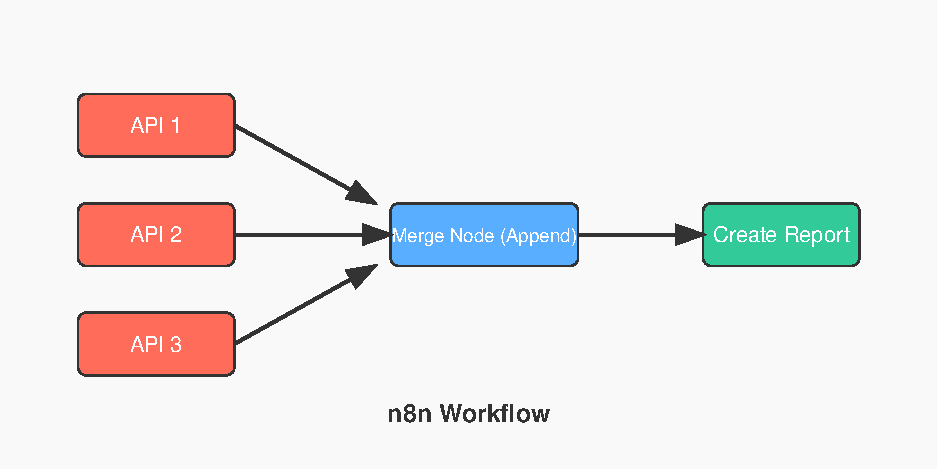
\includegraphics[width=1\linewidth]{Chap1-7/merge.pdf}
    % \caption{Caption}
\end{figure}

Cấu hình Merge Node:
\begin{itemize}
  \item Mode: Append
  \item Output format: Combine data from all inputs into a single array
\end{itemize}

Do n8n hoạt động theo nguyên tắc chạy các luồng từ trên xuống dưới, từ trái sang phải. Vì vậy sẽ không có 2 luồng rẽ nhánh mà cùng chạy và cho kết quả song song, Node merge này sẽ giúp ta làm điều đó. 


Ta lấy một ví dụ như này cho dễ hiểu: một API để truy xuất thông tin đơn hàng, API này cần 2 tham số là user\_id và order\_id được lấy từ bảng users và order. Ta có 2 node để lấy user\_id và order\_id 2 node này nếu trực tiếp đi vào node chứa api thì sẽ gây lỗi do node này chạy trước, node kia chạy sau. Lúc này ta sẽ cần node merger để tổng hợp kết quả từ 2 node đằng trước cùng lúc để truyền vào node chứa api sau đó.

\clearpage
\subsection{Kết hợp IF, Switch và Merge}

Các nút IF, Switch và Merge thường được sử dụng cùng nhau để tạo các workflow phức tạp.

\subsubsection{Ví dụ: Hệ thống xử lý đơn hàng}

Xây dựng workflow xử lý đơn hàng dựa trên tình trạng thanh toán và tồn kho:

\begin{figure}[htbp]
    \centering
    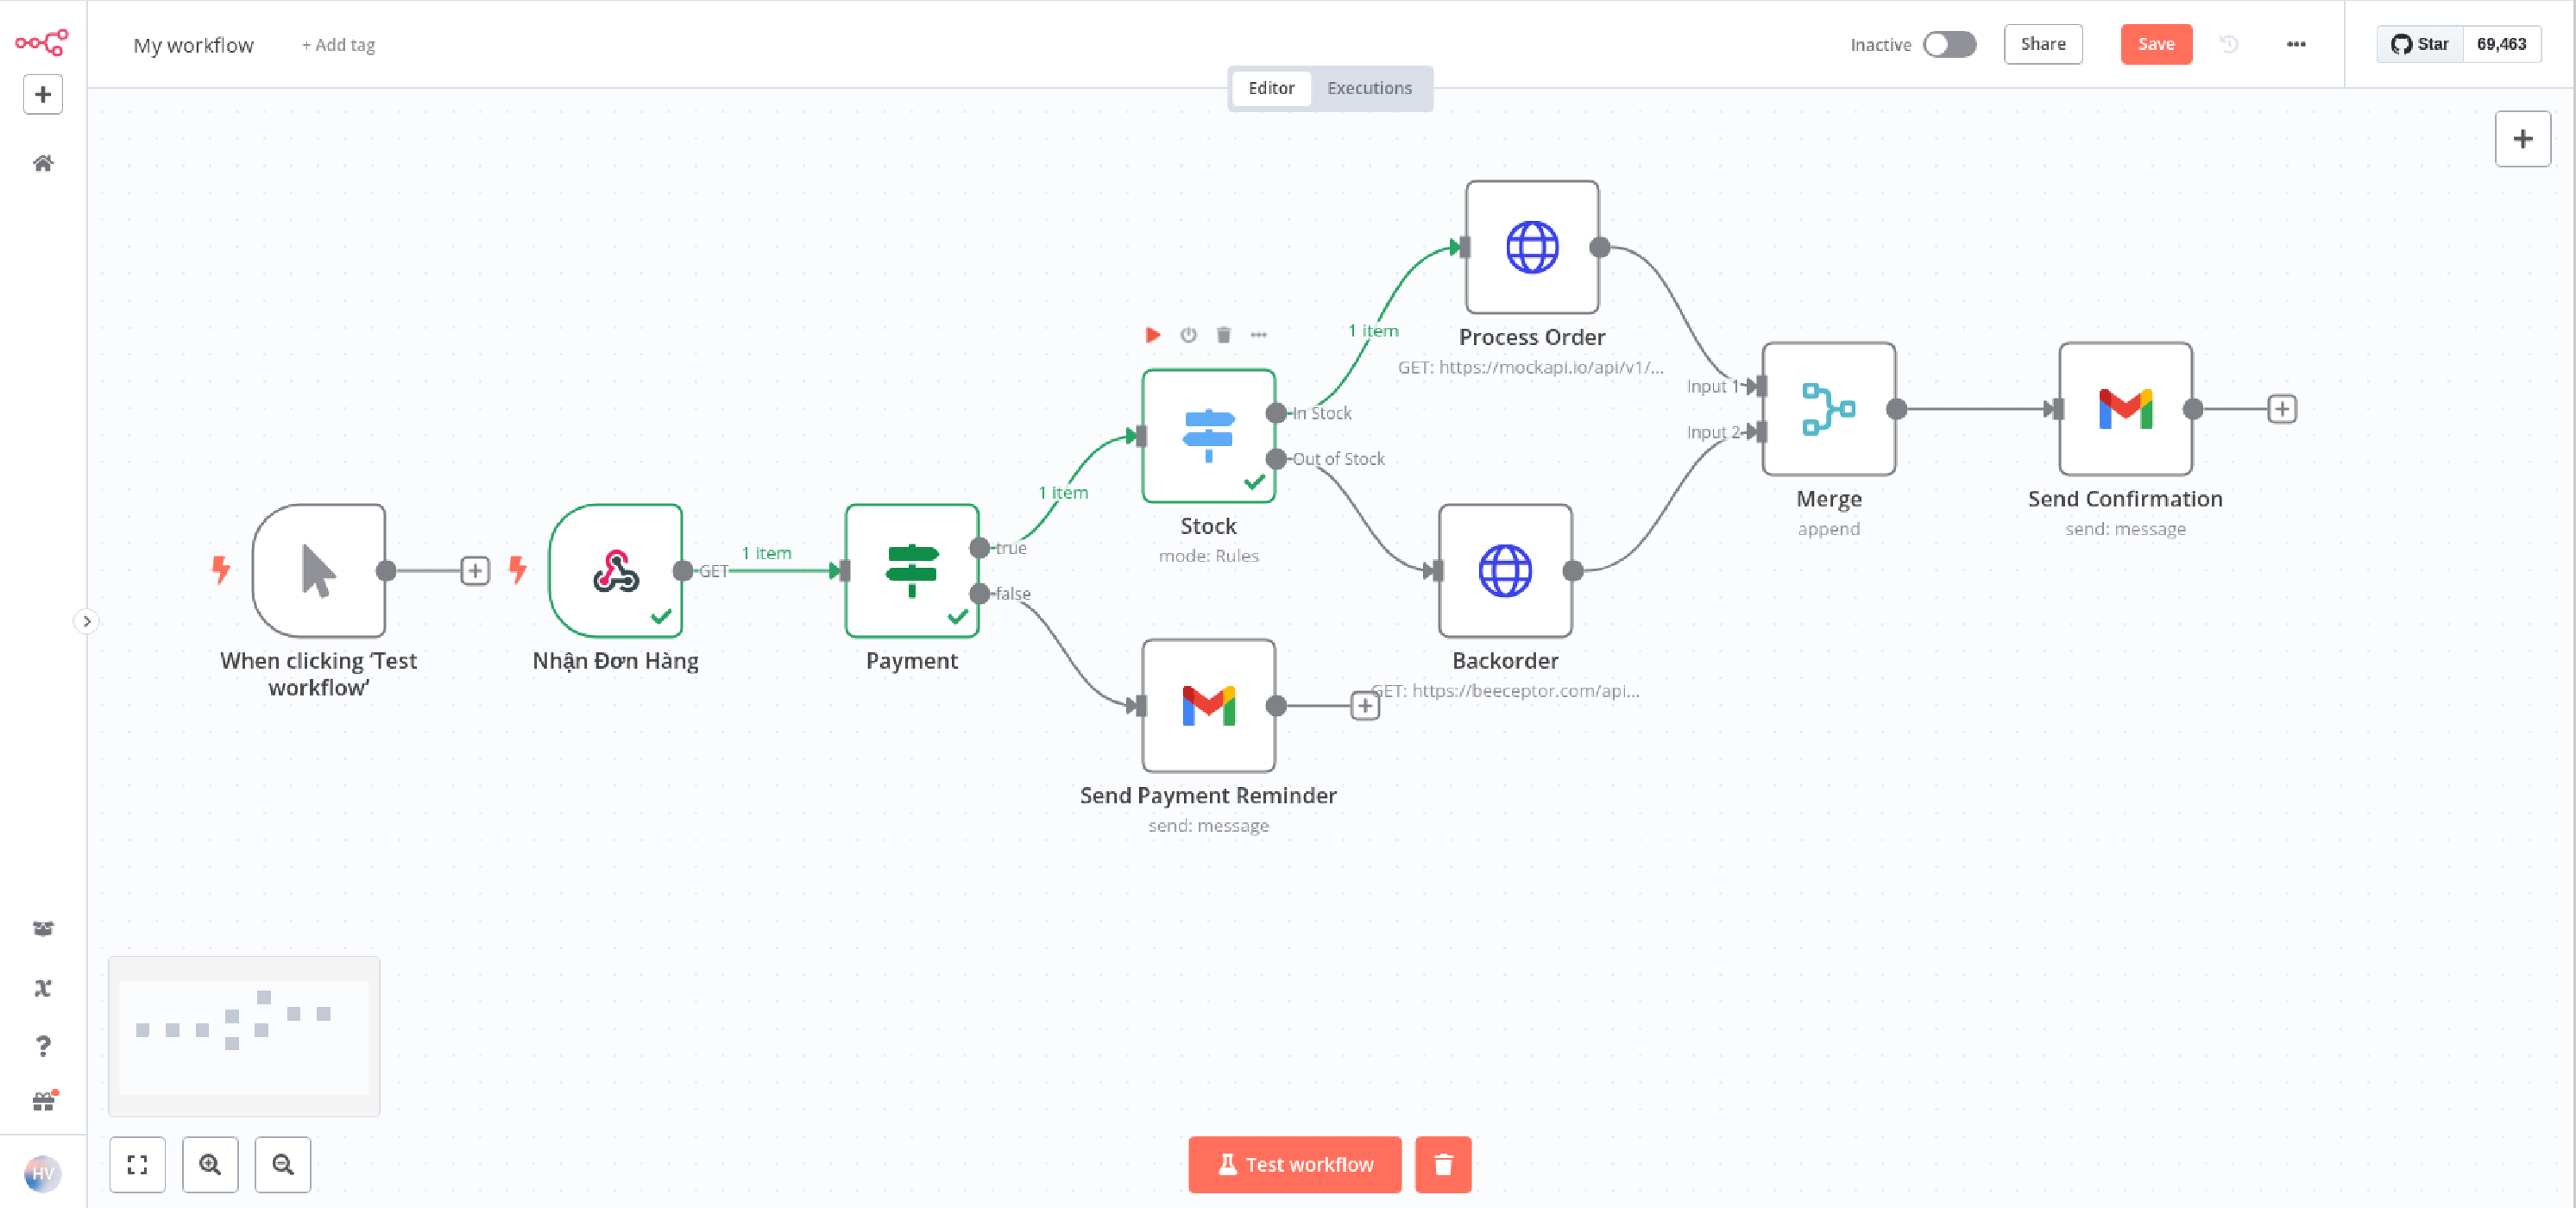
\includegraphics[width=1\linewidth]{Chap1-7/stock.pdf}
    % \caption{Caption}
    % \label{fig:enter-label}
\end{figure}

% \begin{verbatim}
% Order -> IF Node (Payment) -> [True] -> Switch Node (Stock) -> [In Stock] -> Process Order
%                            -> [False] -> Send Payment Reminder

%                                                            -> [Out of Stock] -> Backorder
                                                           
% Process Order -> 
% Backorder    -> Merge Node -> Send Confirmation
% \end{verbatim}

Cấu hình:
\begin{enumerate}
  \item IF Node:
  \begin{itemize}
    \item Điều kiện: \texttt{\{\{\$json["payment\_status"]\}\}} \texttt{equals} \texttt{"paid"}
  \end{itemize}

  \item Switch Node:
  \begin{itemize}
    \item Value: \texttt{\{\{\$json["stock\_status"]\}\}}
    \item Output 1: ``In Stock'', Value ``available''
    \item Output 2: ``Out of Stock'', Value ``unavailable''
  \end{itemize}

  \item Merge Node:
  \begin{itemize}
    \item Mode: Append
    \item Kết hợp cả đơn hàng xử lý thành công và đơn hàng chờ để gửi xác nhận.
  \end{itemize}
\end{enumerate}

\section{Vòng lặp For, While trong n8n}

\subsection{For Loop}

Trong lập trình truyền thống, vòng lặp là kỹ thuật căn bản giúp tự động hóa việc lặp đi lặp lại một hành động với dữ liệu.

Vòng lặp FOR: Lặp qua một tập hợp dữ liệu có số lượng xác định.
Ví dụ: lặp 10 lần, lặp qua danh sách 100 khách hàng.

Cấu trúc phổ biến:

\begin{verbatim}
for (khởi tạo; điều kiện; bước lặp) {
    // hành động
}
\end{verbatim}
Trong n8n, để lặp qua danh sách dữ liệu — tương tự vòng lặp FOR — chúng ta sử dụng node Split In Batches. Trước tiên, hãy học cách "chia để trị" dữ liệu. Trong n8n, node Split In Batches chính là công cụ đắc lực giúp bạn chia nhỏ dữ liệu thành từng phần, đảm bảo workflow vận hành mượt mà và dễ kiểm soát.

\subsubsection{Split In Batches hoạt động như thế nào?}

Hãy tưởng tượng bạn có một danh sách dài khách hàng cần xử lý. Thay vì dồn hết vào một lần — dễ quá tải, dễ lỗi — bạn chia thành từng nhóm nhỏ (batch) và xử lý từng nhóm một cách nhẹ nhàng.

\begin{figure}[htbp]
    \centering
    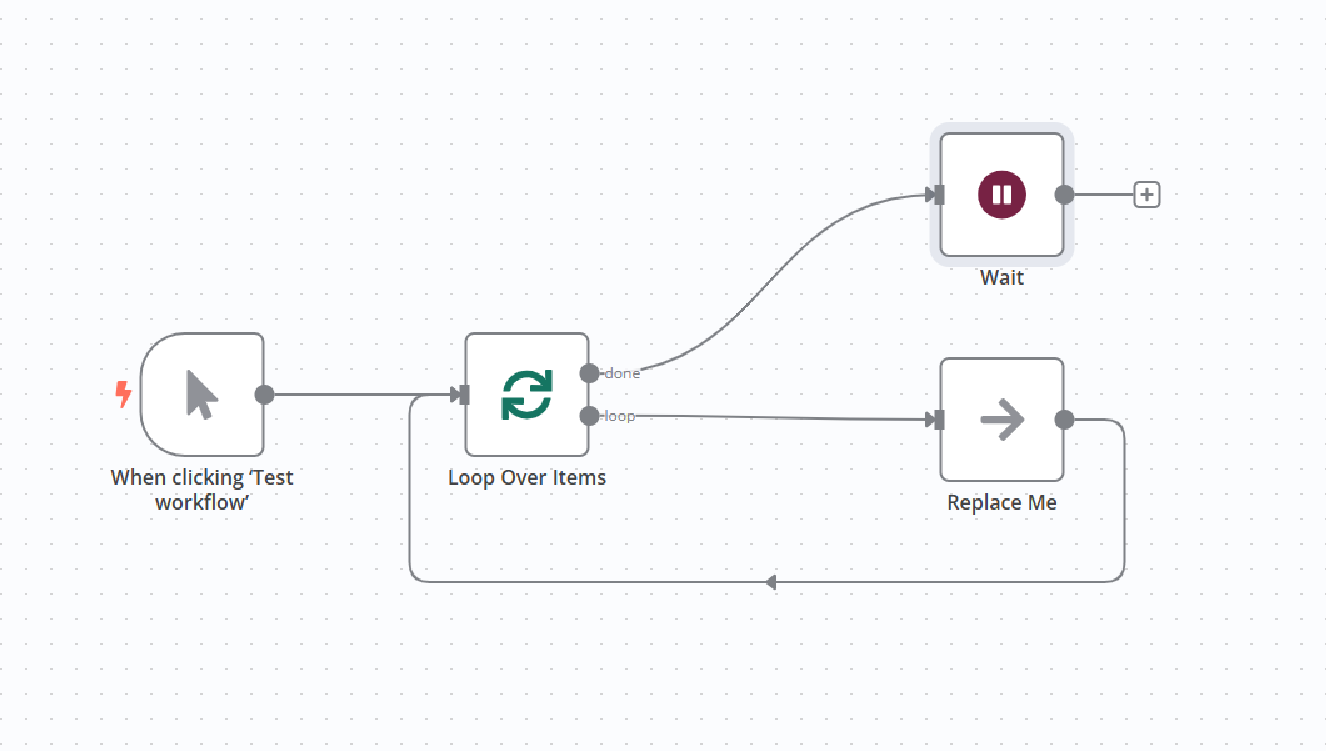
\includegraphics[width=1\linewidth]{Chap1-7/loop.pdf}
    \caption{Split In Batches}
\end{figure}

\subsubsection{Cấu hình Split In Batches}

\begin{enumerate}
  \item \textbf{Thêm Split In Batches vào workflow}:
  \begin{itemize}
    \item Tìm và thêm ``Split In Batches'' từ thư viện nút.
  \end{itemize}

  \item \textbf{Cấu hình kích thước batch}:
  \begin{itemize}
    \item Batch Size: Số lượng mục trong mỗi batch.
    \item Ví dụ: Nếu có 100 mục và batch size là 10, sẽ tạo ra 10 batch.
  \end{itemize}
\end{enumerate}

\textit{Mẹo: Chọn batch size phù hợp để tối ưu tốc độ mà không làm quá tải hệ thống.}

\subsubsection{Ví dụ: Xử lý danh sách khách hàng}

\begin{verbatim}
Database (1000 customers) -> Split In Batches (100) -> Process Each Batch
\end{verbatim}

\subsection{While Loop}
Vòng lặp WHILE: Lặp cho tới khi một điều kiện trở thành sai.
WHILE phù hợp với các tình huống không biết trước số lần lặp, như chờ API trả kết quả.

Cấu trúc:

\begin{verbatim}
while (điều kiện) {
    // hành động
}
\end{verbatim}


Khi học lập trình, chúng ta quen với các vòng lặp như FOR, WHILE, DO-WHILE, hay WHILE-DO. Tuy nhiên, trong n8n — một nền tảng no-code/low-code — không có sẵn một node While hay cấu hình vòng lặp trực tiếp trong một node khác. Không sao hết, thay vào đó, chúng ta hoàn toàn có thể mô phỏng một vòng lặp bằng cách tận dụng đường đi của các node.

\subsubsection{Cách hoạt động của While loop}   

Tận dụng kĩ năng lập trình, các kiến thức về while loop trong ngôn các ngôn ngữ lập trình. Ta sử dụng node điều kiện (ví dụ IF hoặc Switch) để kiểm tra điều kiện lặp, và nếu điều kiện đúng thì tiếp tục đi qua các node xử lý, rồi quay ngược lại node kiểm tra điều kiện. Nếu điều kiện sai thì dừng vòng lặp.

Ta xét workflow minh họa sau:

\begin{figure}[htbp]
    \centering
    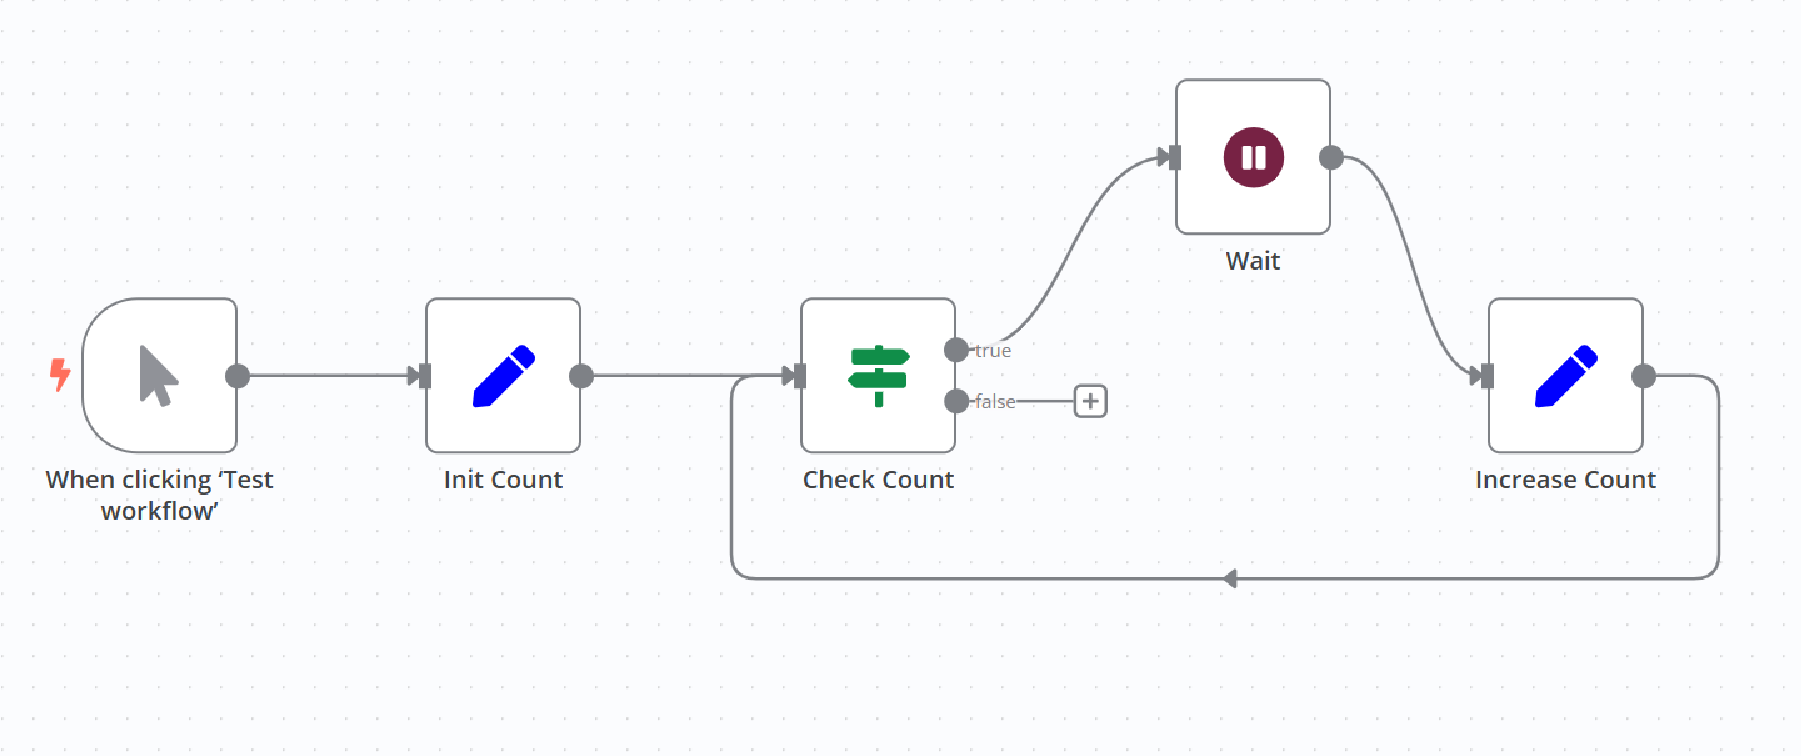
\includegraphics[width=1\linewidth]{Chap1-7/While-loop.pdf}
    \caption{Minh họa while loop}
\end{figure}
Mô tả:
\begin{itemize}
    \item When clicking 'Test workflow': Trigger khởi động workflow.

    \item Init Count: Thiết lập biến count = 0.

    \item Check Count: Kiểm tra nếu count < 5 thì trả về true, ngược lại false.

    \item Nếu true:
\begin{itemize}
    \item Wait: Dừng tạm workflow một khoảng thời gian (ví dụ 1s).

    \item Increase Count: Tăng giá trị count lên 1.

    \item Quay lại node Check Count để kiểm tra lại.

\end{itemize}
    \item Nếu false: workflow kết thúc.

\end{itemize}

Dù n8n không có node WHILE sẵn, nhưng bằng cách thiết kế luồng workflow hợp lý và kết hợp node IF, Wait, và các node xử lý logic khác, bạn hoàn toàn có thể tạo ra vòng lặp WHILE, FOR hay DO-WHILE.

\subsubsection{Ví dụ: Polling API cho đến khi nhận được kết quả}

\begin{verbatim}
While Node -> HTTP Request -> IF (Result Ready) 
 -> [True] -> Exit Loop
 -> [False] -> Wait 1s -> Back to While
\end{verbatim}

Cấu hình:
\begin{itemize}
  \item While Condition: \texttt{\{\{\$json["status"]\}\}} \texttt{not equals} \texttt{"completed"}
  \item HTTP Request: Kiểm tra trạng thái của một tác vụ dài.
  \item IF Node: Kiểm tra xem tác vụ đã hoàn thành chưa.
  \item Wait: Chờ 5 giây trước khi thử lại.
\end{itemize}

\subsection{Kỹ thuật nâng cao: Vòng lặp lồng nhau}

Trong một số trường hợp, bạn có thể cần các vòng lặp lồng nhau để xử lý dữ liệu phức tạp.

\subsubsection{Ví dụ: Xử lý dữ liệu đa cấp}

Xử lý danh sách khách hàng và đơn hàng của họ:

\begin{verbatim}
Database (Customers) -> For Each Customer -> Database (Orders) 

-> For Each Order -> Process Order
\end{verbatim}

Cấu hình:
\begin{enumerate}
  \item For Each Customer:
  \begin{itemize}
    \item Items: \texttt{\{\{\$json["customers"]\}\}}
  \end{itemize}
  
  \item Database (Orders):
  \begin{itemize}
    \item Query: Get orders for the current customer.
  \end{itemize}
  
  \item For Each Order:
  \begin{itemize}
    \item Items: \texttt{\{\{\$json["orders"]\}\}}
  \end{itemize}
  
  \item Process Order:
  \begin{itemize}
    \item Logic xử lý đơn hàng.
  \end{itemize}
\end{enumerate}


\textit{Bạn có thể lặp lồng nhau bao nhiêu tầng tùy ý, miễn workflow hợp lý và được kiểm soát tốt.}

\newpage
\section{Xử lý lỗi trong workflow}
Trong quá trình xây dựng workflow với n8n, lỗi là điều không thể tránh khỏi. Một workflow hoàn chỉnh không chỉ cần chạy đúng khi mọi thứ suôn sẻ mà còn phải biết xử lý tốt các tình huống ngoại lệ để đảm bảo hệ thống vận hành ổn định, giảm thiểu rủi ro gián đoạn.
\subsection{Error Workflow - Xử lý lỗi cơ bản}
\begin{figure}[htbp]
    \centering
    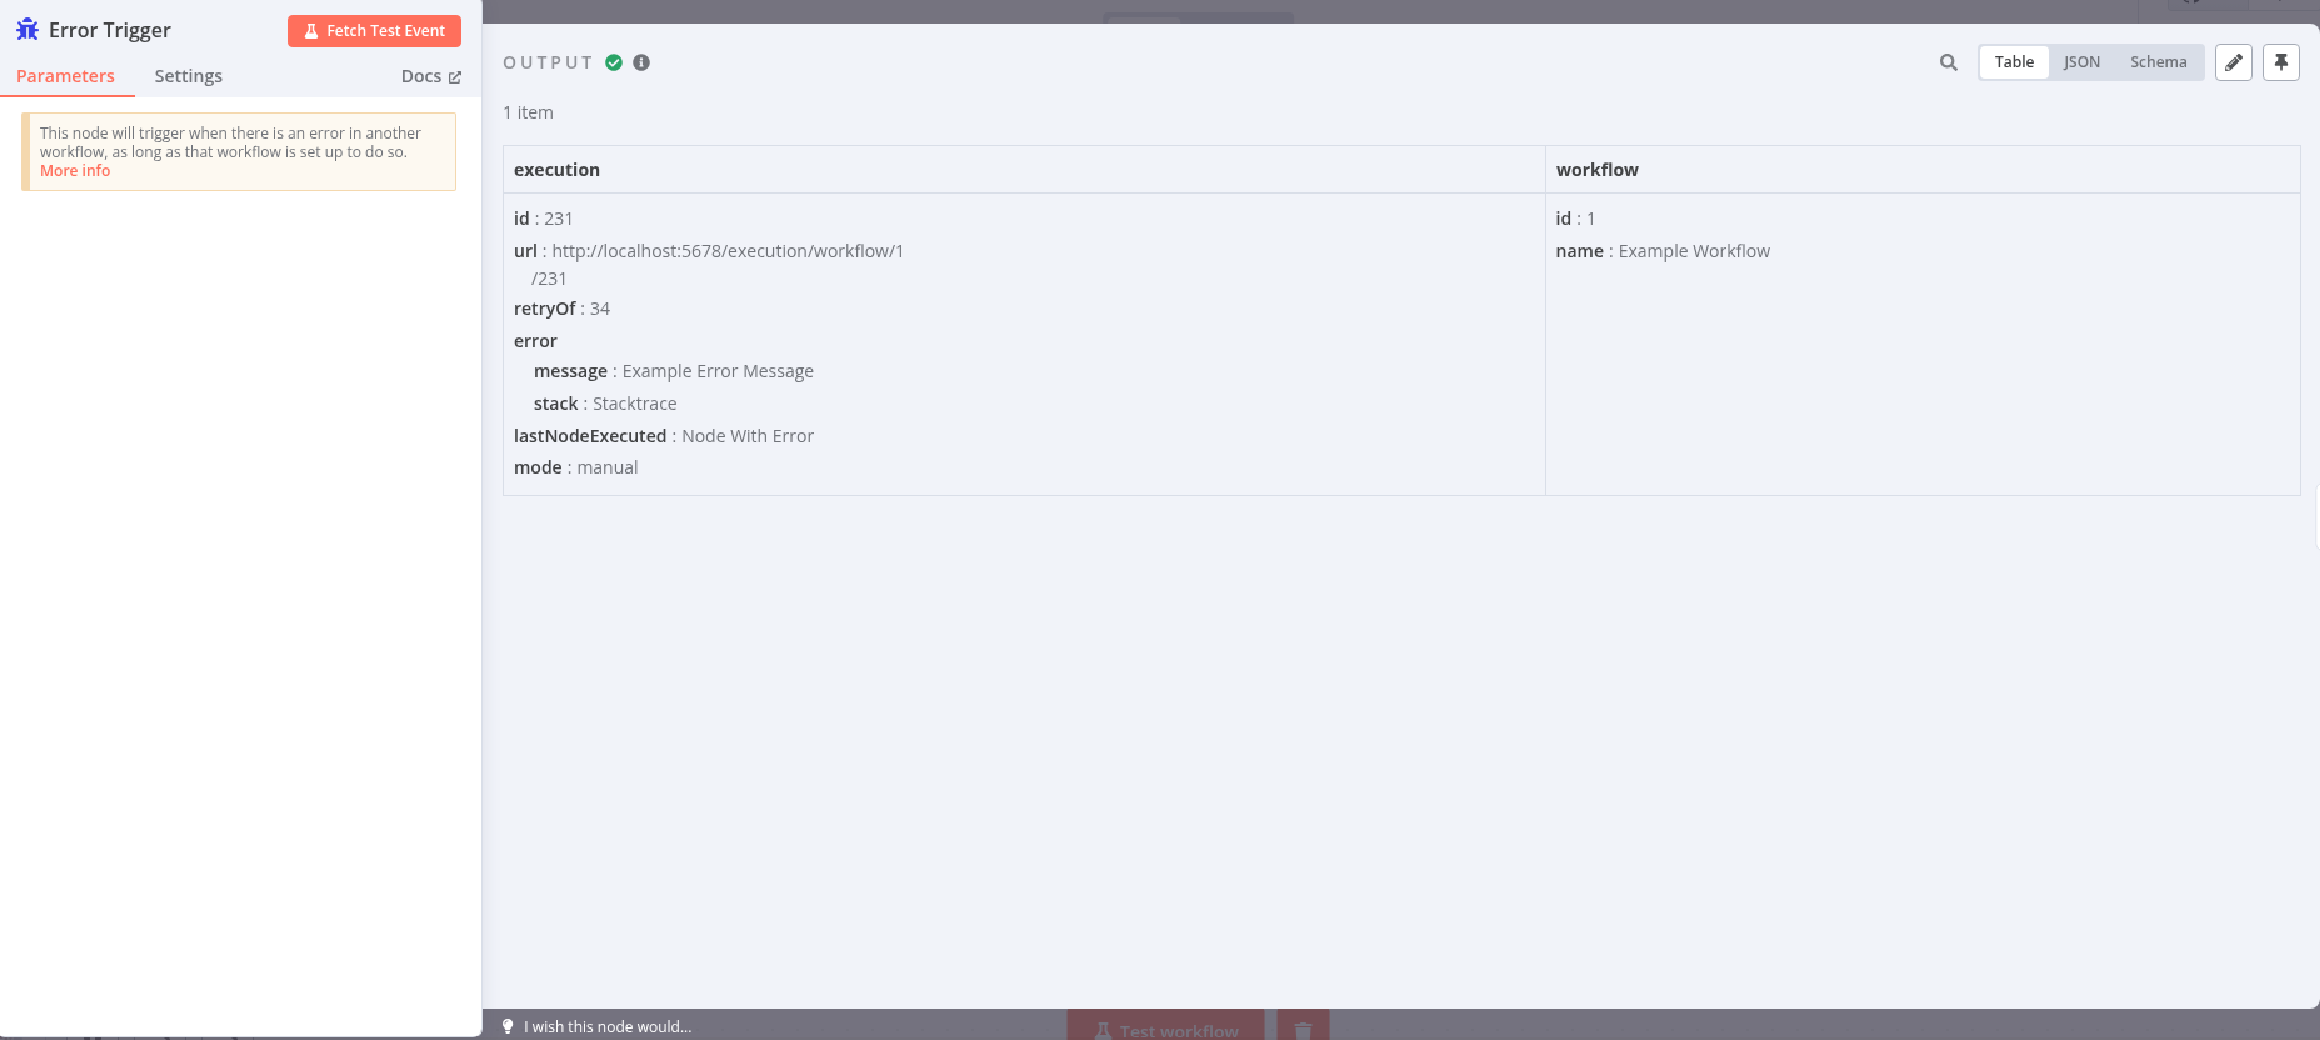
\includegraphics[width=1\linewidth]{Chap1-7/error_event.pdf}
    \caption{Khi một workflow lỗi nó sẽ trả về như này}
\end{figure}

$\rightarrow$ Để đảm bảo hệ thống hoạt động ổn định và có khả năng phục hồi, n8n cung cấp các cơ chế xử lý lỗi hiệu quả.

\subsubsection{Các loại lỗi phổ biến}

\begin{enumerate}
  \item Lỗi kết nối: Không thể kết nối đến API hoặc dịch vụ.
  \item Lỗi xác thực: Các vấn đề về xác thực hoặc ủy quyền.
  \item Lỗi dữ liệu: Dữ liệu không hợp lệ hoặc thiếu.
  \item Lỗi thời gian chờ: Các yêu cầu mất quá nhiều thời gian.
\end{enumerate}

\newpage

\subsubsection{Cấu hình Error Workflow}
\begin{figure}[htbp]
    \centering
    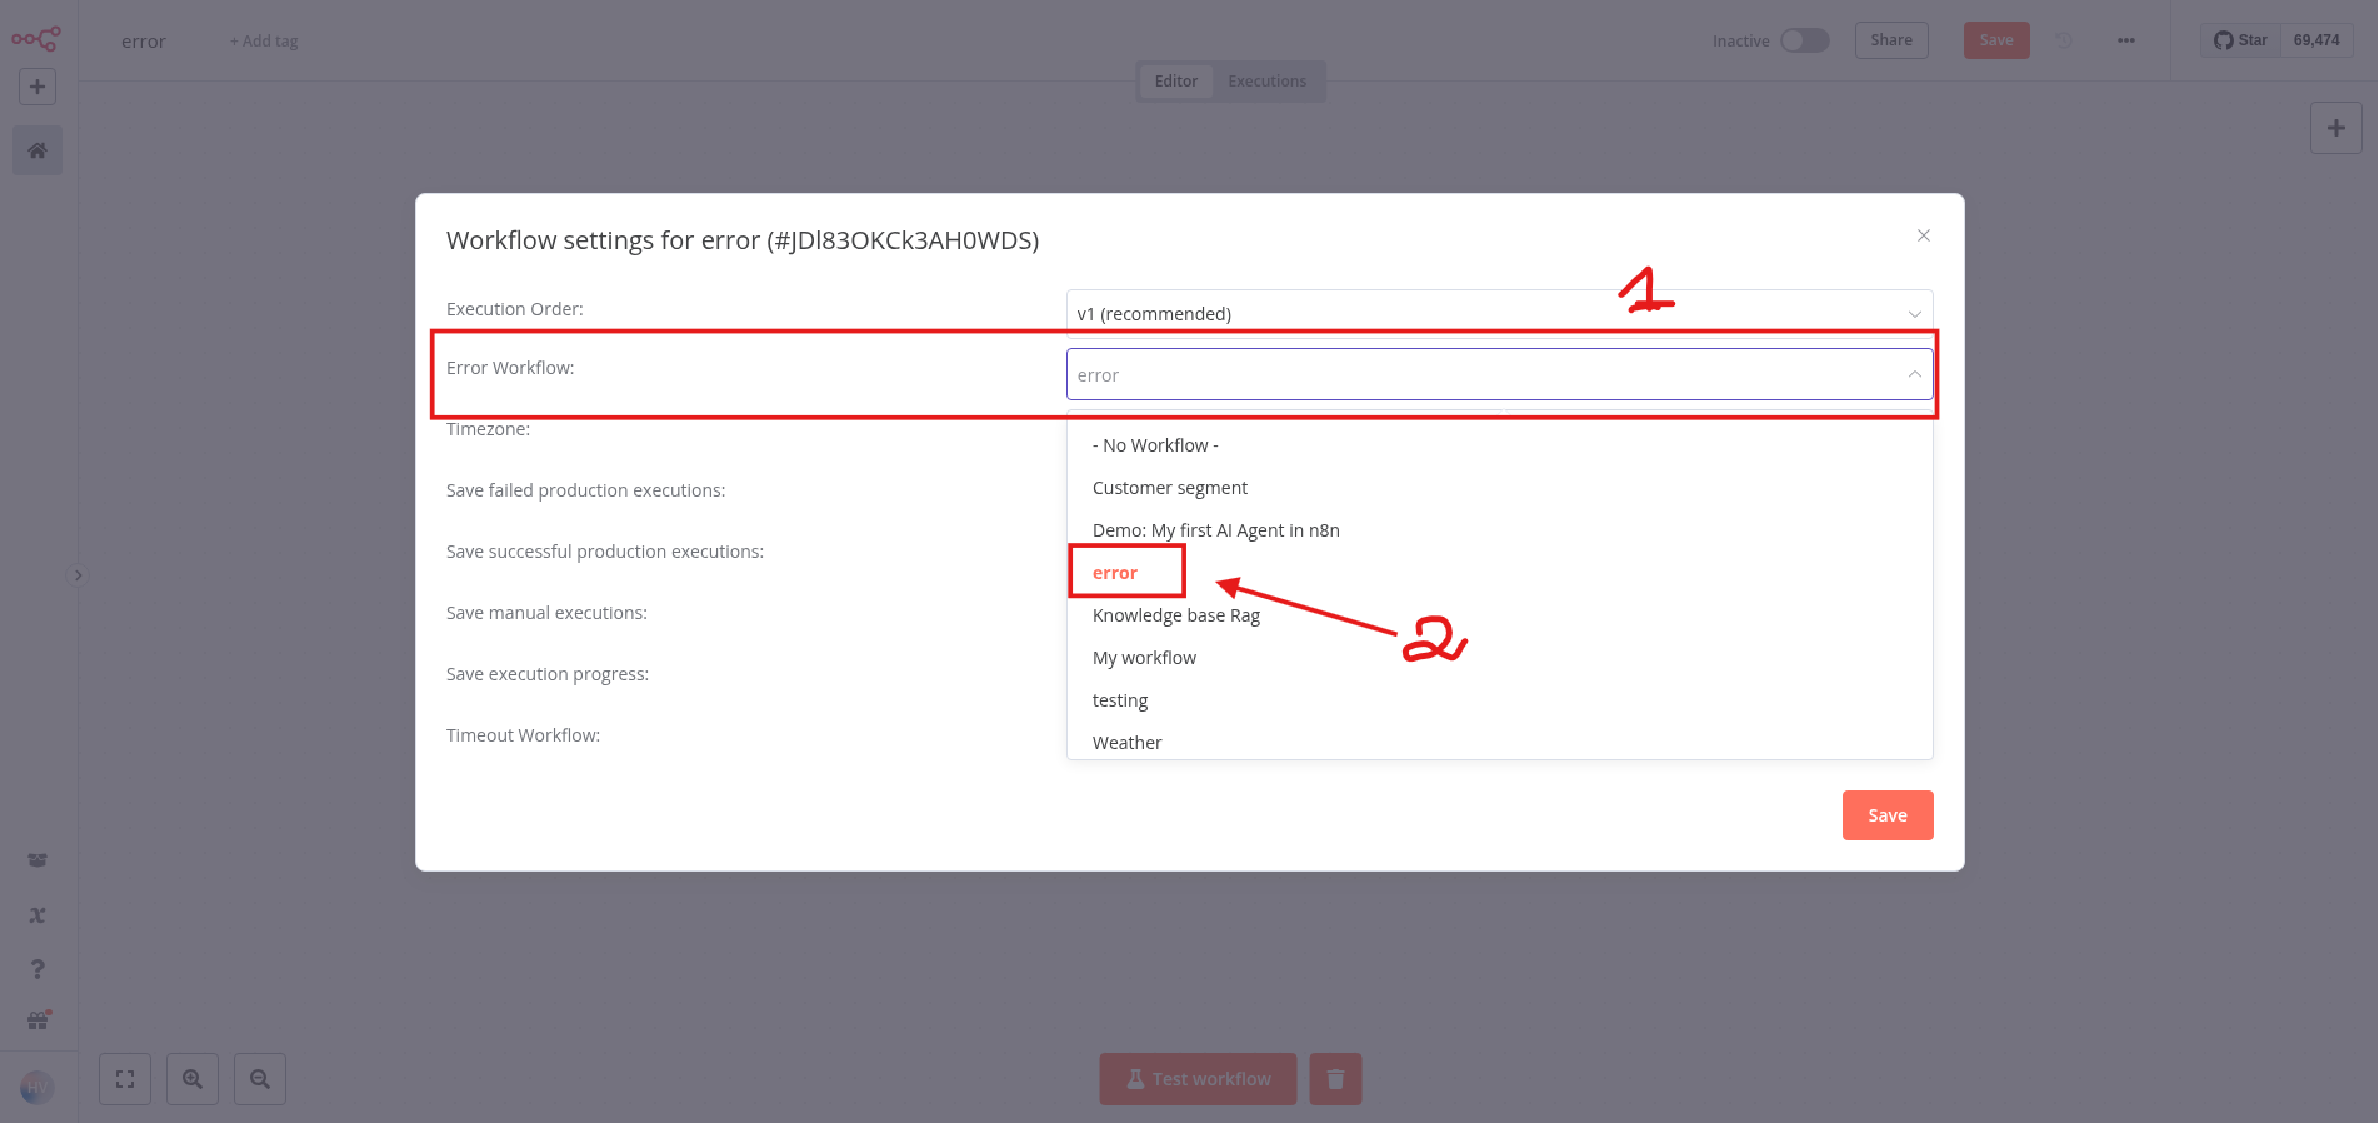
\includegraphics[width=1\linewidth]{Chap1-7/setting_error.pdf}
\end{figure}

N8N cho phép định nghĩa một Error Workflow - một workflow riêng biệt sẽ được kích hoạt khi workflow chính gặp lỗi.

\begin{enumerate}
  \item \textbf{Tạo Error Workflow}:
  \begin{itemize}
    \item Tạo một workflow mới để xử lý lỗi.
    \item Ví dụ: Gửi thông báo, ghi nhật ký lỗi, hoặc thực hiện các bước phục hồi.
  \end{itemize}

  \item \textbf{Kết nối với workflow chính}:
  \begin{itemize}
    \item Trong workflow chính, mở Settings > Error Workflow.
    \item Chọn Error Workflow đã tạo.
  \end{itemize}
\end{enumerate}

\subsection{Error Trigger Node}

Câu chuyện là khi mà workflow nó chạy ổn định mượt mà thì không sao trên thực tế thì lỗi rất nhiều (ae làm dev thì biết nè) chạy nó phải có lúc lỗi lúc không thường do nhiều nguyên nhân. Kiểu mấy tool như Airflow chạy cả năm không sao một ngày đùng phát có lỗi. Mà khi có lỗi thì workflow lỗi nó dùng và không chạy các node tiếp theo. 

$\Rightarrow$ \textit{Cần setup workflow để báo lỗi cho admin vào sửa}

\newpage

Error Trigger Node cho phép bạn bắt đầu một workflow dựa trên lỗi từ workflow khác.

\begin{figure}[htbp]
    \centering
    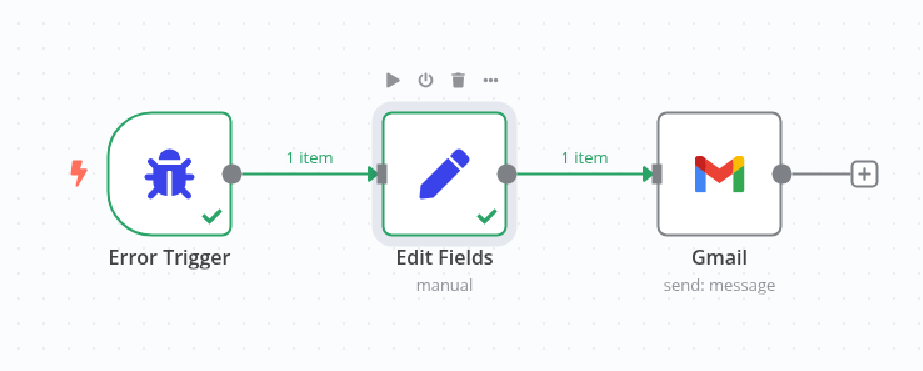
\includegraphics[width=1\linewidth]{Chap1-7/error.pdf}
\end{figure}

\subsubsection{Cấu hình Error Trigger}

\begin{figure}[htbp]
    \centering
    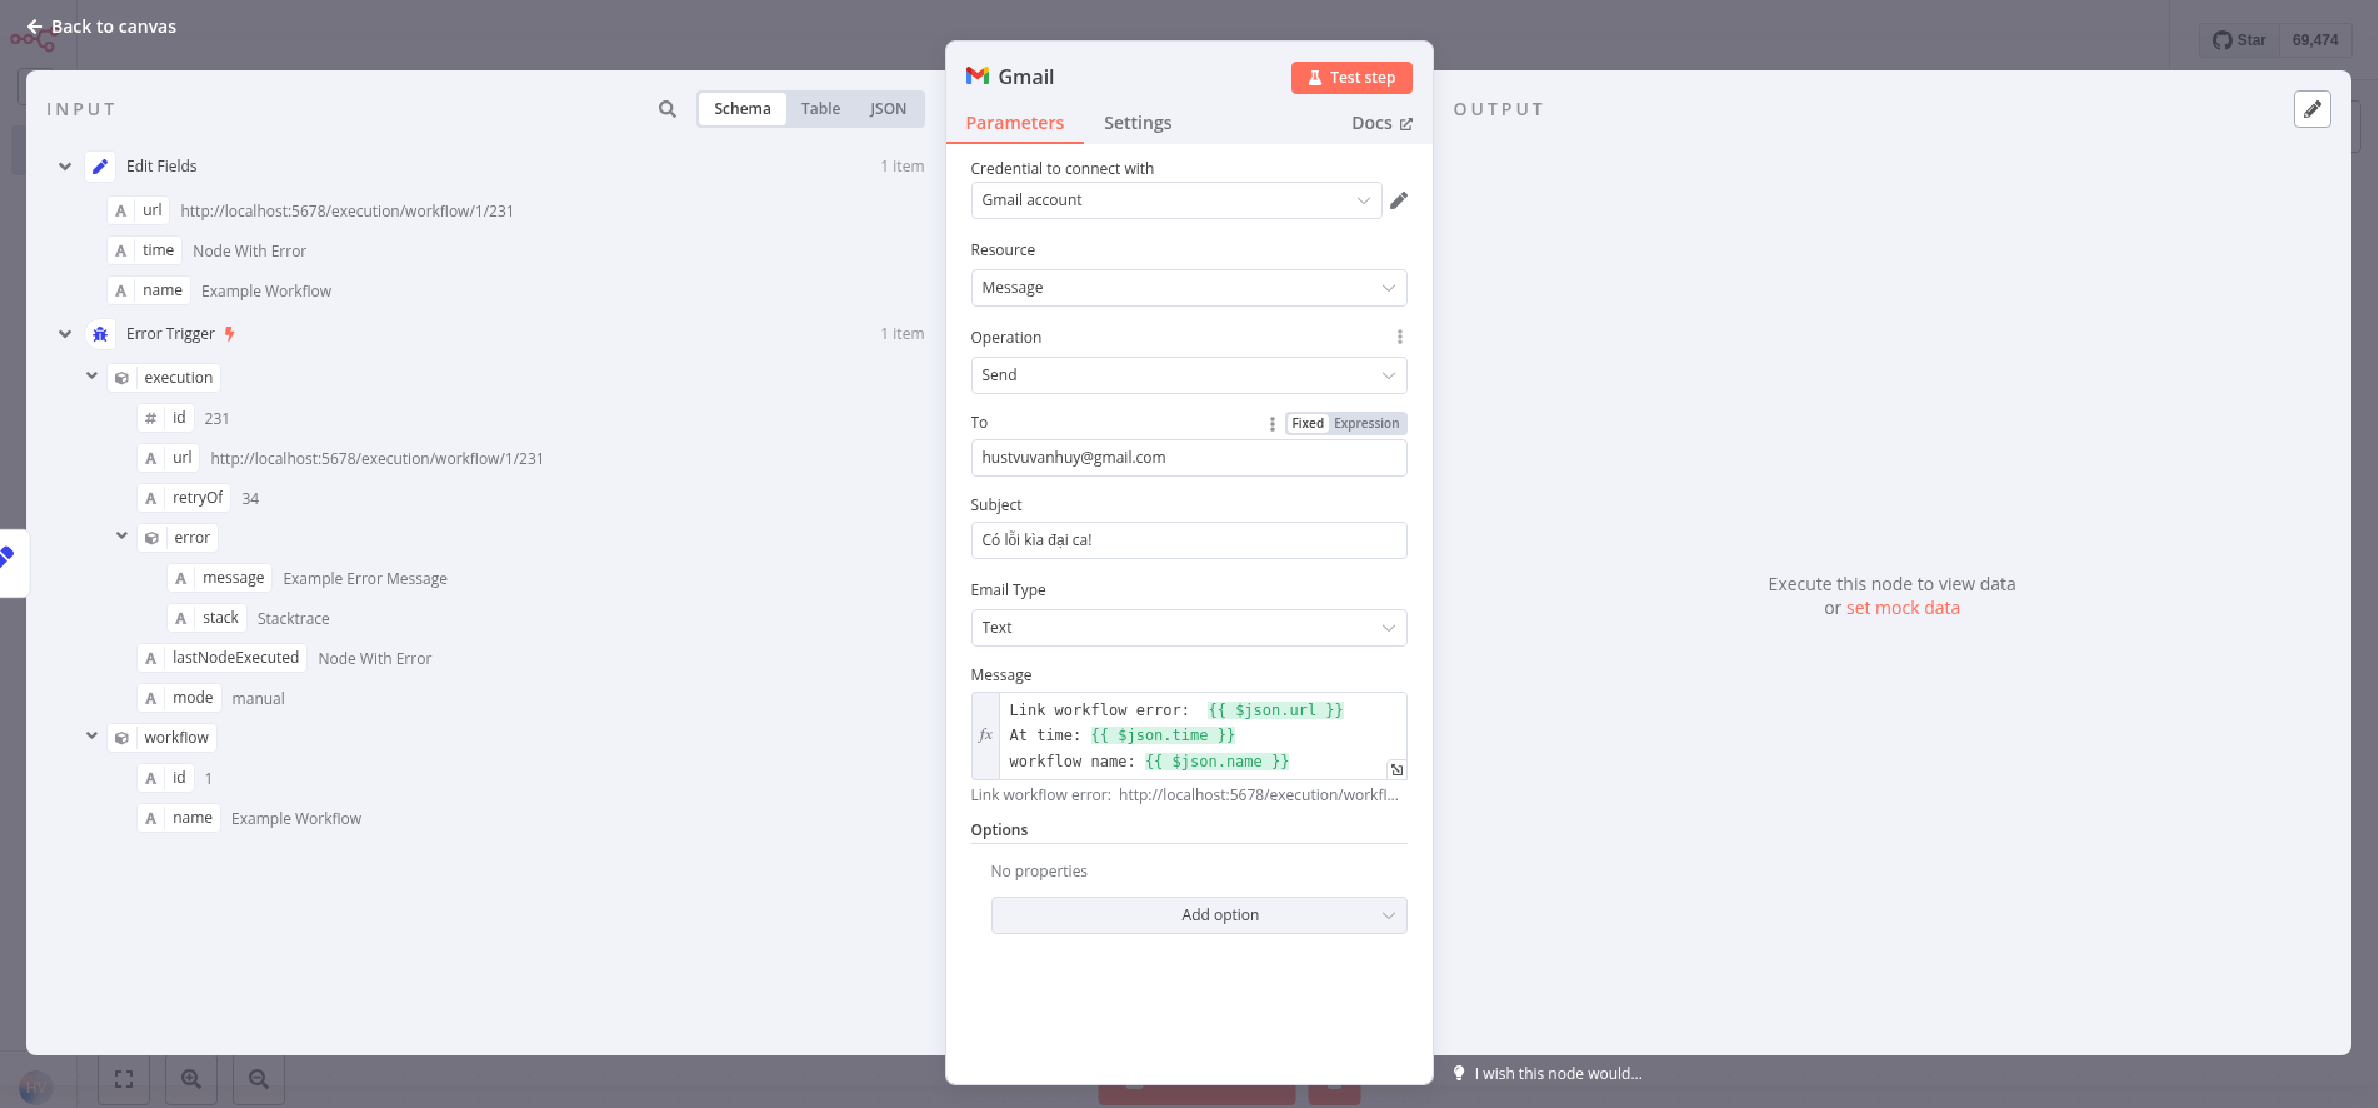
\includegraphics[width=1\linewidth]{Chap1-7/mess_error.pdf}
\end{figure}

\begin{enumerate}
  \item \textbf{Thêm Error Trigger vào Error Workflow}:
  \begin{itemize}
    \item Sử dụng ``Error Trigger'' làm nút bắt đầu.
  \end{itemize}

  \item \textbf{Thiết lập workflow cần theo dõi}:
  \begin{itemize}
    \item Chọn workflow cần được giám sát.
  \end{itemize}

  \item \textbf{Xử lý dữ liệu lỗi}:
  \begin{itemize}
    \item Truy cập thông tin lỗi thông qua \texttt{\{\{\$json["error"]\}\}}.
    \item Truy cập workflow gốc thông qua \texttt{\{\{\$json["workflow"]\}\}}.
    \item Hoàn toàn có thể lưu các lỗi vào sheet để dễ dàng theo dõi.
  \end{itemize}
\end{enumerate}


\subsection{Try/Catch trong n8n}

n8n không có cú pháp Try/Catch giống như các ngôn ngữ lập trình, nhưng bạn có thể mô phỏng hành vi này.

\subsubsection{Cách thực hiện Try/Catch}

Sử dụng kết hợp IF Node, Error Trigger và Function Node:

\begin{verbatim}
-> Function (Try) -> IF (Success) -> [True] -> Tiếp tục workflow
                  -> [False] -> Function (Catch) -> Xử lý lỗi
\end{verbatim}

Cấu hình:
\begin{enumerate}
  \item Function (Try):
  \begin{verbatim}
  try {
    // Mã có thể gây lỗi
    const result = await $items(0).json.riskyOperation();
    return { success: true, data: result };
  } catch (error) {
    return { success: false, error: error.message };
  }
  \end{verbatim}

  \item IF Node:
  \begin{itemize}
    \item Điều kiện: \texttt{\{\{\$json["success"]\}\}} \texttt{equals} \texttt{true}
  \end{itemize}

  \item Function (Catch):
  \begin{verbatim}
  // Xử lý lỗi
  return { error_handled: true, message: "Đã xử lý lỗi: " + $items(0).json.error };
  \end{verbatim}
\end{enumerate}

\newpage
\subsection{Retry khi gặp lỗi}

Thêm khả năng thử lại cho các hoạt động không ổn định như các yêu cầu API.

\subsubsection{Sử dụng vòng lặp và điều kiện để thử lại}

\begin{verbatim}
While Loop -> HTTP Request -> IF (Success) 
 -> [True] -> Exit Loop
 -> [False] -> Function (Retry Logic) -> Back to While
\end{verbatim}

Cấu hình:
\begin{enumerate}
  \item Function (Retry Logic):
  \begin{verbatim}
  // Tăng bộ đếm thử lại
  const retryCount = $items(0).json.retryCount || 0;
  const maxRetries = 3;
  
  if (retryCount < maxRetries) {
    return { retryCount: retryCount + 1, retry: true };
  } else {
    return { retryCount: retryCount, retry: false, error: "Đã vượt quá số lần thử lại" };
  }
  \end{verbatim}

  \item While loop:
  \begin{itemize}
    \item Điều kiện: \texttt{\{\{\$json["retry"]\}\}} \texttt{equals} \texttt{true}
  \end{itemize}
\end{enumerate}

\subsubsection{Ví dụ: Gọi API không ổn định}

\begin{verbatim}
Set (retryCount:0) -> While (retryCount<3) -> HTTP Request -> IF (Success)
 -> [True] -> Exit 
 -> [False] -> Wait -> Increment retryCount
\end{verbatim}
\subsection{Ghi nhật ký và giám sát}

Việc ghi nhật ký đầy đủ là quan trọng để giám sát và gỡ lỗi workflow.

\subsubsection{Thêm ghi nhật ký vào workflow}

\begin{enumerate}
  \item \textbf{Function Node để ghi nhật ký}:
  \begin{verbatim}
  // Ghi nhật ký với dấu thời gian
  const log = {
    timestamp: new Date().toISOString(),
    step: "Processing Customer Data",
    data: $items(0).json
  };
  
  // Truyền cả dữ liệu gốc và thông tin nhật ký
  return { ...item[0].json, log };
  \end{verbatim}

  \item \textbf{Tích hợp với hệ thống giám sát}:
  \begin{itemize}
    \item Gửi nhật ký đến Slack, email, hoặc hệ thống giám sát.
    \item Lưu trữ nhật ký trong cơ sở dữ liệu để phân tích sau.
  \end{itemize}
\end{enumerate}

\subsubsection{Ví dụ: Workflow có khả năng phục hồi đầy đủ}

\begin{verbatim}
Trigger -> 
  Function (Log Start) -> 
    Try Process -> 
      IF (Success) -> 
        [True] -> Function (Log Success) -> Continue
        [False] -> Function (Log Error) -> Error Handling -> Retry Logic
\end{verbatim}

\section{Tổng kết}

Trong chương này, chúng ta đã tìm hiểu về:

\begin{enumerate}
  \item Nút điều kiện (IF, Switch) để tạo các luồng xử lý động dựa trên dữ liệu.
  \item Merge Node để kết hợp dữ liệu từ nhiều nhánh.
  \item Vòng lặp (Each Item, For Each, While) để xử lý nhiều mục dữ liệu.
  \item Xử lý lỗi để tạo các workflow có khả năng phục hồi.
\end{enumerate}

Việc kết hợp các kỹ thuật này sẽ cho phép bạn xây dựng các workflow phức tạp và mạnh mẽ, có thể xử lý các tình huống thực tế đa dạng.

\newpage
\section{Bài tập thực hành}

\begin{enumerate}
  \item Tạo một workflow sử dụng IF Node để phân loại email dựa trên nội dung.
  \item Xây dựng một workflow sử dụng For Each để gửi thông báo tùy chỉnh cho từng thành viên trong nhóm.
  \item Tạo một Error Workflow để thông báo và ghi nhật ký khi workflow chính gặp sự cố.
\end{enumerate}